% Generated by figures/gen_phase1_figures.py
\begin{figure*}[t]
    \centering
    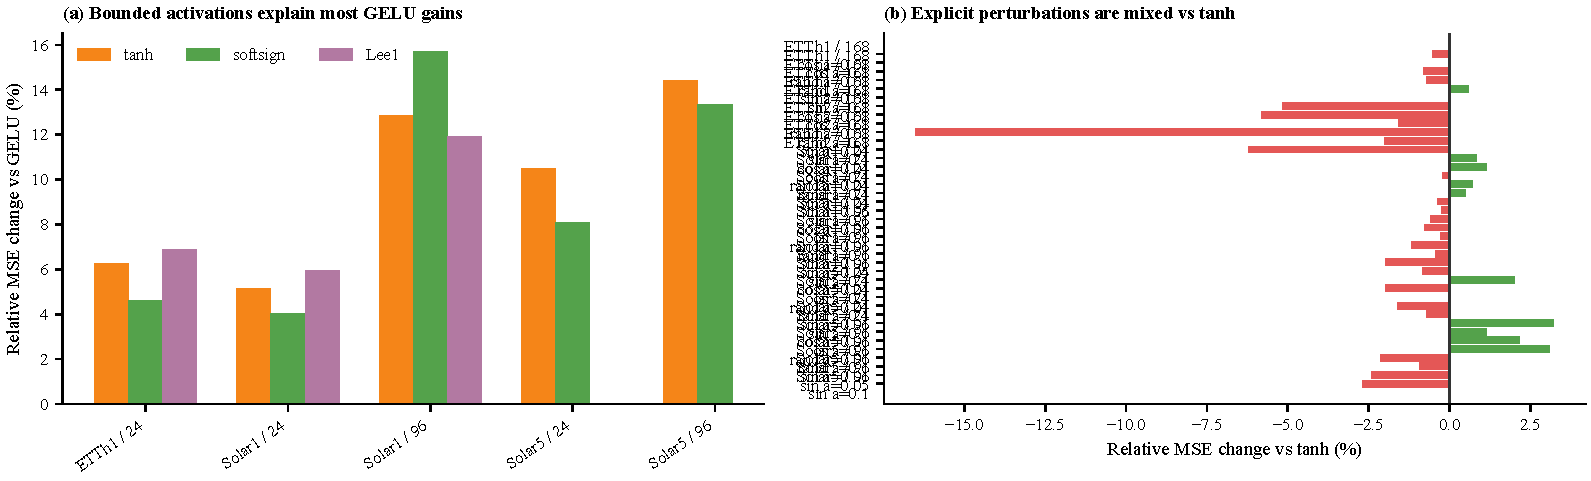
\includegraphics[width=\textwidth]{figures/fig1_activation_effects.pdf}
    \caption{Activation-only changes produce measurable Informer forecasting differences. (a) Bounded sign-preserving activations explain the strongest current gains over GELU. (b) Explicit perturbations around \texttt{tanh} are mixed and should not be treated as globally reliable.}
    \label{fig:activation_effects}
\end{figure*}

\begin{figure}[t]
    \centering
    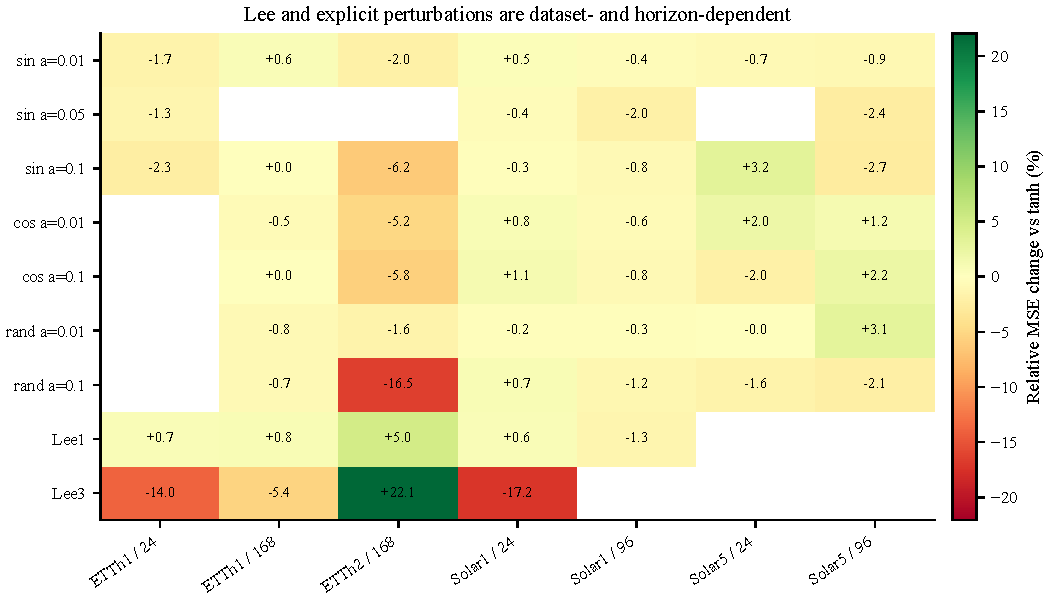
\includegraphics[width=\linewidth]{figures/fig2_tanh_specificity_heatmap.pdf}
    \caption{Specificity tests against \texttt{tanh}. Lee and explicit oscillatory perturbations are strongly dataset- and horizon-dependent.}
    \label{fig:tanh_specificity}
\end{figure}

\begin{figure*}[t]
    \centering
    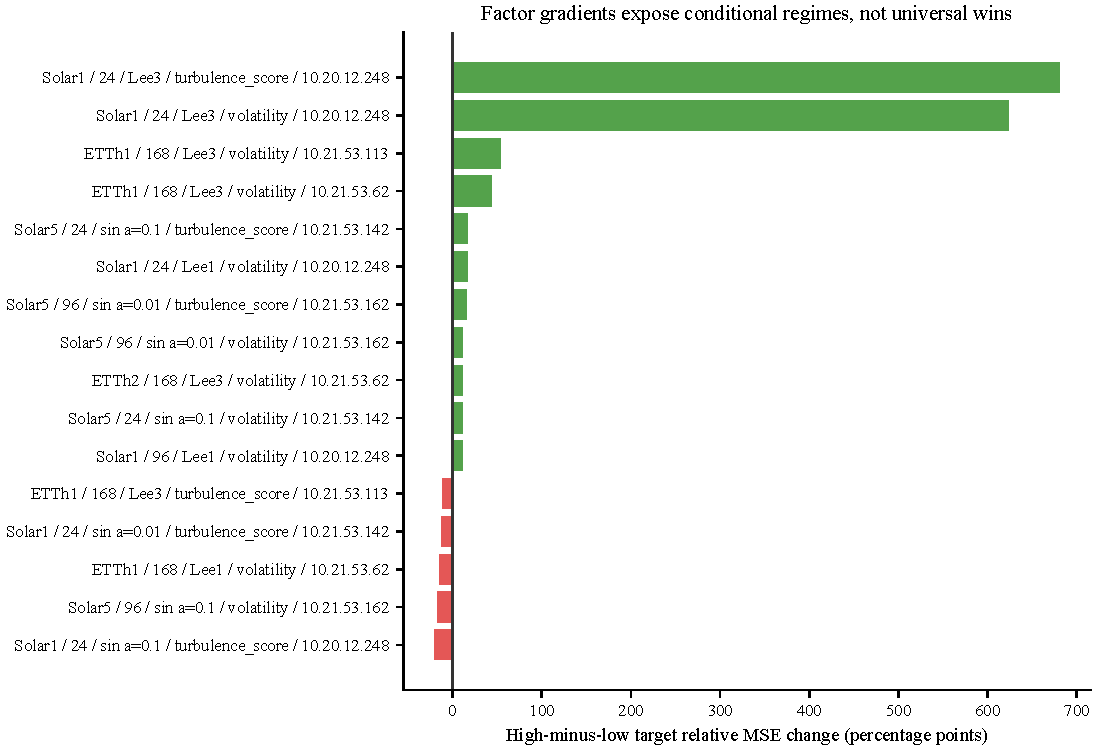
\includegraphics[width=\textwidth]{figures/fig3_factor_gradients.pdf}
    \caption{Input-factor gradients reveal conditional regimes. Positive values mean the high factor bin gains more than the low factor bin, but this diagnostic must be interpreted with global MSE and seed win rates.}
    \label{fig:factor_gradients}
\end{figure*}
